\documentclass{article}
\usepackage{array, booktabs, graphicx, apacite, setspace, tocbibind, lipsum}
\usepackage[titletoc,toc,title]{appendix}
\usepackage[toc,section=section]{glossaries}

% format appendix numbering
\renewcommand\appendix{\par
  \setcounter{section}{0}
  \setcounter{subsection}{0}
  \setcounter{figure}{0}
  \setcounter{table}{0}
  \renewcommand\thesection{Appendix \Alph{section}}
  \renewcommand\thefigure{\Alph{section}\arabic{figure}}
  \renewcommand\thetable{\Alph{section}\arabic{table}}
}

% glossary and definitions
\makenoidxglossaries

\newglossaryentry{Lorem}{name={Lorem},description={hold back, hold fast, take hold of, seize, catch }}

% renames "Contents" to "Table of Contents"
\renewcommand\contentsname{Table of Contents}

\begin{document}

% ---- FRONT MATTER ---- %

% title page w/o page numbers

\title{Formal APA Report Template}
\author{Charles Clayton}
\date{\today}
\maketitle

\thispagestyle{empty}

\pagenumbering{roman}
\setcounter{page}{0}

% auto-generated front matter w/ roman page numbering

\singlespacing			\pagebreak
\tableofcontents		\pagebreak

\listoffigures		
\listoftables			\pagebreak

\printnoidxglossaries	\pagebreak

% ---- MAIN MATTER ---- %

\pagenumbering{arabic}
\onehalfspacing
\section{Introduction}

\gls{Lorem} ipsum \cite{einstein}.

\subsection{History}
\lipsum[2]

\subsection{Present Day}
\lipsum[2]

\begin{table}[ht]
  \centering
  \caption{Table without vertical lines}
  \begin{tabular}{>{\centering\bfseries}m{1in} >{\centering}m{1in} >{\centering}m{1in} >{\centering\arraybackslash}m{1in}}
    \toprule
    Letter & \textbf{Dates} & \textbf{Number} & \textbf{Note} \\ 
    \midrule
	$x$ & 5-Mar-2016 & 1 & do \\
	$y$ & 5-Mar-2016 & 2 & re \\
	$z$ & 5-Mar-2016 & 3 & mi \\
	\bottomrule
  \end{tabular}
\end{table}

\subsection{Future}
\lipsum[2]

\section{Discussion} 
\lipsum[2]

\begin{equation}
\int_{0}^{2\pi} \rho^2 d\rho
\end{equation}

\subsection{Design} 
\lipsum[2]

\subsubsection{Details}
\lipsum[2]
\cite{knuth-fa}

\subsubsection{Schematic}
\lipsum[2]
\begin{figure}[ht!]
\centering
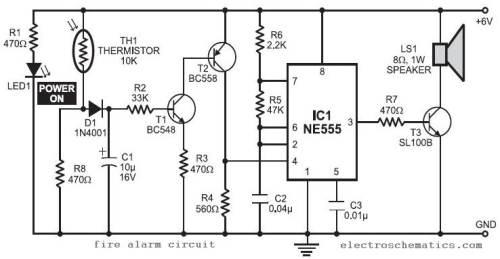
\includegraphics[width=100mm]{Images/schematic.png}
\caption{Schematic image}
\end{figure}

\section{Conclusion}
\lipsum[2]


% ---- BACK MATTER ---- %

% bibliography
\doublespacing
\clearpage
\bibliography{references}
\bibliographystyle{apacite} 
\pagebreak


\appendix
\section*{Appendix}
\addcontentsline{toc}{section}{Appendix}
\renewcommand{\thesubsection}{\Alph{subsection}}

\subsection{Solved Problems}
\lipsum[2]


\end{document}